\chapter{Why this book?\clabel{Why}}
%\section{Summary}
%\seclabel{Summary}
{\it In this introductory chapter we lay the conceptual foundation for the rest 
of what we have to say about redeveloping economic theory. In \secref{The_game} we play a simple coin-toss game and analyze it 
numerically, by Monte Carlo simulation, and analytically, with pen and paper. The game motivates the 
introduction of the expectation value and the time average, which in turn 
lead to a discussion of ergodic properties. The ergodicity question  -- whether time averages are identical to expectation values -- will turn out to be the key to our redevelopment of formal economics. This is because ergodicity hadn't been established as a concept when the original formalism was developed. We note the importance of rates as ergodic observables.
This section also introduces the concepts of a random variable, a stochastic process, scalars as representations of transitive preferences, logarithms and exponentials, and dimensional analysis.

In \secref{Brownian_motion} we notice that wealth on logarithmic scales follows a random walk in our game, and we relate this to Brownian motion, as the continuous-time limit of the random walk. This allows us to introduce Brownian motion and its scaling properties that are robust enough to yield insights into more complicated models.

Finally, we ask in \secref{Geometric_Brownian} what wealth in our game is doing in the continuum limit but on linear scales. This takes us to geometric Brownian motion, which will be our starting point for much of the rest of these lectures. We derive ensemble-average and time-average growth rates for geometric Brownian motion, by explicitly taking the continuous-time limit, and then state the key result of \Ito calculus, \eref{Ito_process} and \eref{Ito}, which allows an easier derivation of these growth rates and will be relied on in later chapters.

Some historical perspective is provided to understand the prevalence or
absence of key concepts in modern economic theory and other fields.
The emphasis is on introducing key concepts and useful machinery, with more formal treatments and applications
in later chapters.}
\newpage

\section{The game}
\seclabel{The_game}
Imagine we offer you the following game: we toss a coin, and if it comes 
up heads we increase your monetary wealth by 50\%; if 
it comes up tails we reduce your wealth by 40\%. We're not only 
doing this once, we will do it many times, for example 
once per week for the rest of your life. Would you accept 
the rules of our game? Would you submit your wealth to 
the dynamic our game will impose on it?

Your answer to this question is up to you and will be 
influenced by many factors, such as the importance 
you attach to wealth that can be measured in monetary 
terms, whether you like the thrill of gambling, your 
religion and moral convictions and so on.

In these notes we will mostly ignore these factors.
We will build an extremely simple model of your 
wealth, which will lead to an extremely simple and 
powerful model of the way you make decisions that affect 
your wealth. We are interested in analyzing the 
game mathematically, which requires a translation 
of the game into mathematics. We choose the 
following translation: we introduce the key 
variable, $\x(\t)$, which we refer to as ``wealth''. 
We refer to $\t$ as ``time''. It should be kept in mind that
``wealth'' and ``time'' are just names that we've given to 
mathematical objects. We have chosen these names because
we want to compare the behaviour of the mathematical
objects to the behaviour of wealth over time, but
we emphasize that we're building a model -- whether we write $\x(\t)$, 
or $\text{wealth}(\text{time})$, or \smiley(\lightning) makes no difference to the mathematics. 

The usefulness of our model will be different in different circumstances, 
ranging from completely meaningless to very helpful. There is no 
substitute for careful consideration of any given situation, and
labeling mathematical objects in one way or another is certainly none.

Having got these words of warning out of the way, we define our 
model\footnote{For those in the know: ``our'' coin toss is a discrete version of geometric Brownian motion, the workhorse model of financial mathematics and much more.} of the dynamics of your wealth under the rules we just specified. 
At regular intervals of duration $\dt$ we randomly generate a 
factor $\gr(\t)$ with each possible value
$\gr_i\in \{0.6, 1.5\}$ occurring with probability 1/2, 

\be 
\gr(\t) = \begin{cases}
0.6 &\text{with probability  1/2}\\
1.5 &\text{with probability 1/2}
\end{cases}
\elabel{law}
\ee
and multiply current wealth by that factor, so that
\be
\x(\t+\dt)=\gr(\t)\x(\t).
\elabel{gamble}
\ee

We have good reasons to suspect that this model will do something interesting. It's not just a silly game because it has one important property: it's multiplicative. Every time the coin is tossed, wealth is {\it multiplied} by one of the two possible factors. This introduces a reference point, or state-dependence, of the absolute size of the change. Processes with this property are very common in nature -- the amount of anything that reproduces changes in proportion to what's already there. In the absence of other constraints, such as limited resources, this applies to the dynamics of the biomass of a cell culture. In fact, life itself has been defined as that which produces more of itself \cite{Morowitz1992}: life and evolution begin with the minimal chemical structure that can copy itself. The rest, in a sense, is details. We will see, especially in \cref{Interactions}, how multiplicativity generates interesting structure in -- including but not limited to -- economics.

Without discussing in depth how realistic a representation of your 
wealth this model is (for instance your non-gambling related 
income and spending are not represented in the model),
 and without discussing whether randomness truly exists and 
what the meaning of a probability is, we simply switch on a 
computer and simulate what might happen. You may have many 
good ideas of how to analyze our game with pen and paper, 
but we will just generate possible trajectories of your wealth 
and pretend we know nothing about mathematics or 
economic theory. \Fref{1_1} is a trajectory of your wealth, 
according to our computer model as it might evolve over 
the course of 52 time steps (corresponding to one year given our 
original setup).

\begin{figure}[h!]
\begin{picture}(200,230)(0,0)
    \put(0,0){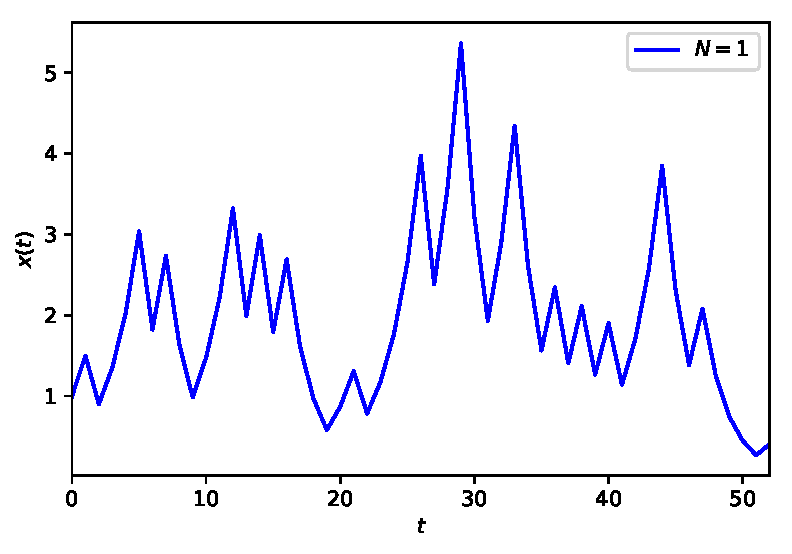
\includegraphics[width=\textwidth]{./chapter_tools/figs/x_of_t_lin_1.pdf}}
\end{picture}
\caption{Wealth $\x(\t)$ resulting from a computer simulation of our game, as specified by \eref{law} and \eref{gamble}, for 52 time steps (corresponding to one year in the given setup).}
\flabel{1_1}
\end{figure}


A cursory glance at the trajectory does not reveal much structure. 
Of course there are regularities, for instance at each time step 
$\x(\t)$ changes, but no trend is discernible -- does this trajectory 
have a tendency to go up, does it have a tendency to go down? 
Neither? What are we to learn from this simulation? Perhaps we 
conclude that playing the game for a year is quite risky, but is the 
risk worth taking? 

\subsection{Averaging over many trials}
The trajectory in \fref{1_1} doesn't tell us much about overall tendencies.
There is too much noise to discern a clear signal. A common 
strategy for getting rid of noise is to try again. And then try again and
again, and look at what happens on average. 
An example of the technique is Shannon's error-correcting code:
instead of sending the message $0$ (or $1$), send the relevant digit 3 times. The recipient averages over the received digits and takes the closest possibility. If one out of three digits was miscommunicated because of noise, the code nonetheless recovers the original message: averaging gets rid of noise.
%For example, this is 
%very successful in imaging -- the 2014 Nobel Prize in chemistry 
%was awarded for a technique that takes a noisy image again and 
%again. By averaging over many images the noise is reduced and 
%\href{https://en.wikipedia.org/wiki/Super-resolution_microscopy#Stochastic_functional_techniques}{a resolution beyond the diffraction limit is achieved}.

So let's try this in our case and see if we can make sense of the game.
In \fref{1_2} we average over a finite number, $N$, of
trajectories. We call a collection of trajectories an ensemble. We shall see that in the limit $N\to\infty$ the ensemble average converges to the expectation value, and indeed the terms ``ensemble average'' and ``expectation value'' are synonyms. To avoid confusion we will be explicit when $N$ is finite: in \fref{1_2} we plot ``finite-ensemble averages.''
\begin{defn}{Finite-ensemble average} The finite-ensemble average of the quantity 
$z$ at a given time $\t$ is
\be
\ave{\z(\t)}_{\N}=\frac{1}{\N}\sum_{\gi=1}^{\N} \z_{\gi}(\t),
\elabel{f_ens}
\ee 
where $\gi$ indexes a particular realization of $\z(\t)$ and $\N$ is the
number of realizations included in the average.
\end{defn}
\begin{figure}[h!]
\begin{picture}(200,200)(0,0)
    \put(-100,0){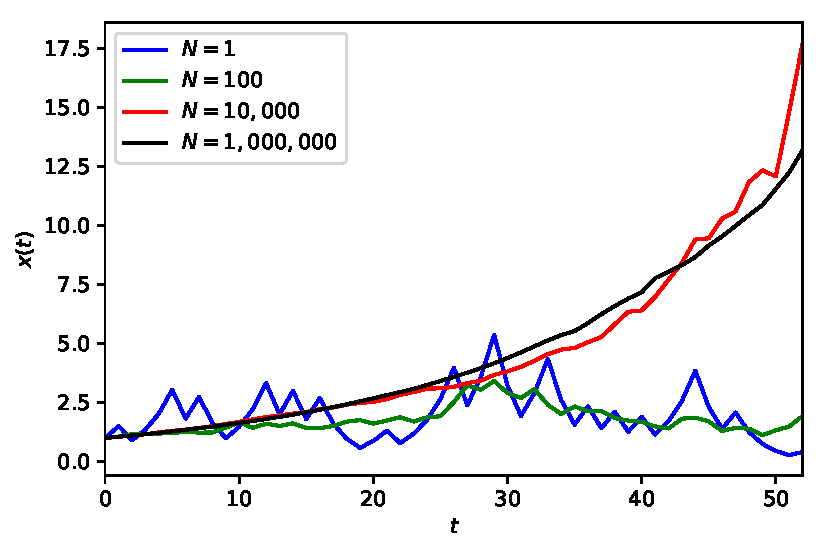
\includegraphics[width=0.8\textwidth]{./chapter_tools/figs/x_of_t_lin.pdf}}
  \put(-50,60){(A)}
  \put(180,0){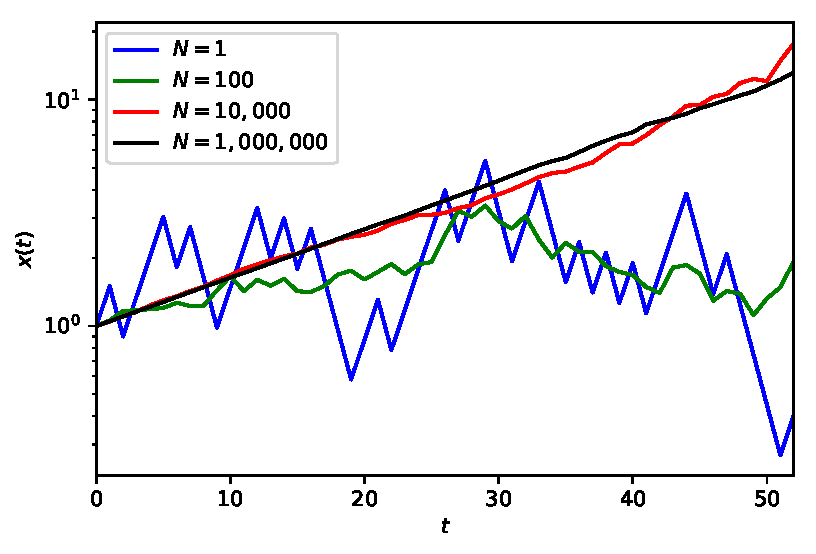
\includegraphics[width=0.8\textwidth]{./chapter_tools/figs/x_of_t_log.pdf}}
  \put(230,60){(B)}  
\end{picture}
\caption{Finite-ensemble averages $\ave{\x(\t)}_{\N}$ for ensemble sizes $\N=1, 
10^2, 
10^4, 10^6$. The noise in the finite-ensemble average diminishes systematically as $\N$ increases. 
(A) on linear scales the multiplicative (non-linear) nature of the process is apparent, (B) on logarithmic scales the multiplicative process is additive in time, and the finite-ensemble average for $\N=10^6$ is a straight line except for small fluctuations.}
\flabel{1_2}
\end{figure}
\FloatBarrier
As expected, the more 
trajectories are included in the average, the smaller the fluctuations of 
that average. For $\N=10^6$ hardly any fluctuations are visible. Since the 
noise-free trajectory points up it is tempting to conclude that my own wealth will similarly go up and  conclude that the risk 
of the game is worth taking. This reasoning has dominated economic 
theory for about 350 years now. But it is flawed. The correction of this flaw and its far-reaching consequences constitute our research program.

\subsection{Averaging over time}
Does our analysis necessitate the conclusion that the gamble is worth taking? 
Of course it doesn't, otherwise we wouldn't be belabouring this point. 
 Our critique will focus on the type of averaging we have applied -- we didn't play the game many times
in a row as would correspond to the real-world situation of repeating the game once a week for the rest of your life. 
Instead we played the game many times in parallel, which corresponds to a different setup\footnote{This different setup could be realised by splitting your wealth into $\N$ equal parts and betting each part in a different sequence of independent coin tosses. But the rules of our game as we defined it don't allow that. Another interesting setup allows the gambler to choose what proportion of his wealth he wants to wager. These conditions were studied by \person{Kelly} \cite{Kelly1956} and are known to every professional poker player. In the present setup, betting $1/4$ of your wealth in each coin toss will lead to the fastest possible growth if you're allowed to choose your wager. You can think of the proportion not wagered as frozen in time: it ensures that, to some extent, you can restore the conditions before the coin toss, which is a bit like allowing you to step back in time.}.

We therefore try a different analysis. \Fref{1_3} shows another simulation of your wealth. This time we don't show an average over many trajectories but a simulation of a single trajectory
over a long time. Noise is removed also in this case but in a different way: to capture visually what 
happens over a long time we have to zoom out -- more time has to be represented by 
the same amount of space on the page. In the process of this zooming-out, small 
short-time fluctuations will be diminished. Eventually the noise will be removed from the system 
just by the passage of time.

\begin{figure}[h!]
\begin{picture}(200,200)(0,0)
    \put(-100,0){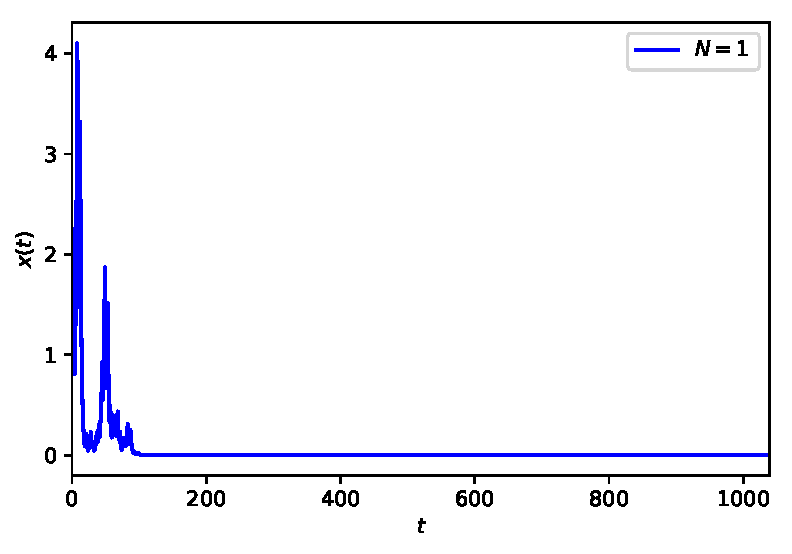
\includegraphics[width=0.75\textwidth]{./chapter_tools/figs/x_of_t_lin_20_year.pdf}}
  \put(-50,50){(A)}
  \put(180,0){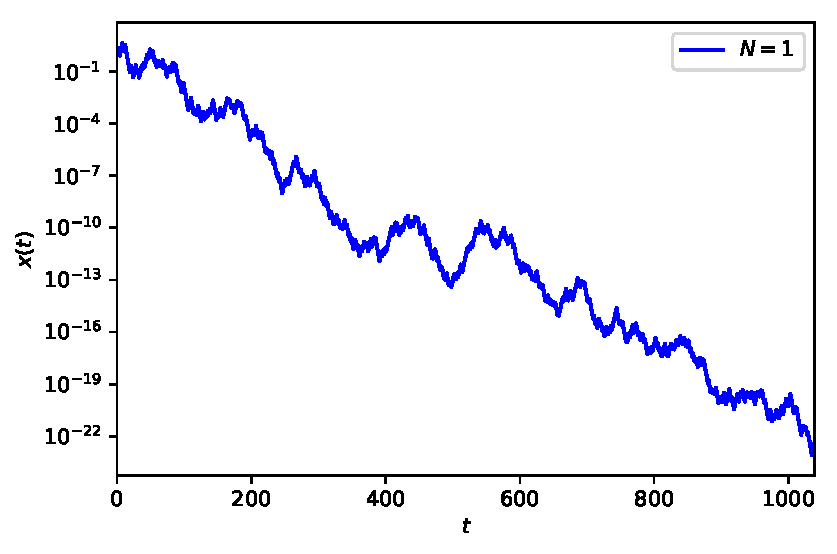
\includegraphics[width=0.8\textwidth]{./chapter_tools/figs/x_of_t_log_20_year.pdf}}
  \put(230,50){(B)}  
\end{picture}
\caption{Single trajectory over 1,040 time steps, corresponding to 20 years 
in our 
setup. (A) on linear scales all we see is wealth quickly dropping to zero, (B) logarithmic scales are more appropriate for the multiplicative process and reveal systematic exponential decay.}
\flabel{1_3}
\end{figure}
\FloatBarrier

The trajectory in \fref{1_3} is, of course, random, but the apparent trend emerging from the randomness 
strongly suggests that our initial analysis in \fref{1_2} does not reflect what happens over time in a single system. 
%Jumping ahead a little, we reveal that this is indeed the case. If it seems counter-intuitive then this is 
%because our intuition is built on so-called ``ergodic processes'', whereas $\x$ is non-ergodic. We will say
%more about this in \secref{Ergodic_observables}.
Several important messages can be derived from the observation that an individual trajectory grows 
more slowly (or decays faster) over time than an average of a large ensemble. 

\begin{enumerate}
\item
An individual whose wealth follows \eref{gamble} will make poor decisions if he uses the 
finite-ensemble average of wealth as an indication of what is likely to happen to his own wealth.
\item
The performance of the average (or aggregate) wealth of a large group of individuals differs systematically from 
the performance of an individual's wealth. In our case large-group wealth grows (think \GDP), whereas 
individual wealth decays.
\item
For point 2 to be possible, \ie for the average to outperform the typical individual, wealth must 
become increasingly concentrated in a 
few extremely rich individuals. The wealth of the richest individuals must be so large that the average becomes 
dominated by it, so that the average can grow although almost everyone's wealth decays. Inequality 
increases in our system.
\end{enumerate}

The two methods we've used to eliminate the noise from our system
are well known. The first method is closely related to the mathematical object called the
``expectation value,'' and the second is closely related to the object called the ``time average.''

\section*{Summary of \cref{Why}}
Suppressed.
%In this chapter we have introduced the following key concepts:
%\bi
%\item[Random variable]
%A random variable $Y$ is a set of pairs of possible values and  corresponding probabilities, $Y=\{(y_1, p_1),(y_2, p_2)...\}$.
%The sets may be discrete or continuous. We stressed that a random variable is an a-temporal concept. It's just a bunch of possible values and their weights (probabilities). In real life we often this of generating instances of random variables as time passes, but this is not part of the formal definition of a random variable.
%
%\item[Expectation value]
%The expectation value of a random variable is the weighted sum $\ave{Y}=\int y \mathcal{P}_Y(y) dy$, where $\mathcal{P}_Y$ has atomic point masses in the discrete case, which means we can express the integral as $\ave{Y}=\sum_i y_i p_i$.
%
%The expectation value is also called the ensemble average, which reflects a physical interpretation: imagine (infinitely) many possible worlds, identical safe for the value taken by the the random variable $Y$. Those values are represented in the superverse of many worlds in proportion to their probabilties. Averaging $y$ over the ensemble of universes then gives the expectation value.
%\ei